The Drucker-Prager yield function is given by the function $f$:
\[
f = p \sin\phi + c\cos \phi - \tau
\]
where $\tau$ is the square root of the second invariant of the deviatoric stress.
We have
\[
p=\frac{1}{2}(\sigma_1+\sigma_3) 
\]
and 
\[
\tau = \frac{1}{2}(\sigma_1-\sigma_3)
\]
Inserting these into $f$ yields:
\[
f= \frac{1}{2}(\sigma_1+\sigma_3) \sin\phi + c \cos\phi - \frac{1}{2}(\sigma_1-\sigma_3)
\]
The yield condition $f=0$ can be reworked as follows:
\[
\sigma_1 - \frac{1 + \sin\phi}{1-\sin\phi} \sigma_3 - 2 \frac{\cos \phi}{1-\sin\phi} c = 0
\]
The third term can further be modified as follows:
\[
\frac{\cos \phi}{1-\sin\phi}
=\frac{\sqrt{1-\sin^2 \phi}}{\sqrt{(1-\sin\phi)^2}}
=\frac{\sqrt{(1-\sin \phi)(1+\sin\phi)}}{\sqrt{(1-\sin\phi)^2}}
=\sqrt{
\frac{1+\sin\phi}{1-\sin\phi}
}
\]
Finally, we define $N_\phi$ as follows 
\[
N_\phi=\frac{1+\sin \phi}{1-\sin\phi}
\]
so that the yield condition becomes:
\[
\sigma_1 - N_\phi \sigma_3 - 2 \sqrt{N_\phi} c = 0
\]
which is Eq.~3 of the article by Choi \& Petersen \cite{chpe15}.

This paper offers a solution to the problem of the angle of shear bands in 
geodynamic models. The underlying idea is based on simple modifications 
brought to existing incompressible flow codes. Note that the codes
featured in that paper also implemented elastic behaviour but this can 
be easily switched off by setting $Z=1$ in their equations.

Their plasticity implementation starts with a modification of the 
continuity equation:
\[
\vec\nabla\cdot\vec\upnu = R = 2 \sin\psi \, \dot{\varepsilon}_p
\]
where $R$ is the dilation rate, $\Psi$ is the dilation angle 
and $\dot{\varepsilon}_p$ is the square root of 
the second invariant of the plastic strain rate.

Under this assumption, the deviatoric strain rate tensor is given by
\[
\dot{\bm \varepsilon}^d(\vec\upnu)
= \dot{\bm \varepsilon}(\vec\upnu)- \frac{1}{3} Tr[\dot{\bm \varepsilon}(\vec\upnu)] {\bm 1}
= \dot{\bm \varepsilon}(\vec\upnu)- \frac{1}{3} \vec\nabla\cdot\vec\upnu \; {\bm 1}
= \dot{\bm \varepsilon}(\vec\upnu)- \frac{1}{3} R \; {\bm 1}
\]
Turning now to the momentum conservation equation:
\begin{eqnarray}
-\vec\nabla p + \vec\nabla \cdot {\bm \tau} 
&=& -\vec\nabla p + \vec\nabla \cdot (2 \eta \dot{\bm \varepsilon}^d(\vec\upnu)) \nonumber \\
&=& -\vec\nabla p + \vec\nabla \cdot \left[ 2 \eta \left(\dot{\bm \varepsilon}(\vec\upnu)- \frac{1}{3} R \; {\bm 1}\right) \right] \nonumber\\
&=& -\vec\nabla p 
+ \vec\nabla \cdot \left( 2 \eta \dot{\bm \varepsilon}(\vec\upnu)\right) -\frac{2}{3} \vec\nabla(\eta R) 
\label{chpeform}
\end{eqnarray}
The last term is then an addition to the right hand side of the momentum equation 
and its weak form is as follows:
\[
\vec f' 
= \int_\Omega N_v \frac{2}{3} \vec\nabla(\eta R) dV
= \frac{4}{3} \sin \Psi \int_\Omega N_v \vec\nabla(\eta \dot{\bm \varepsilon}_p) dV
\]
This formulation proves to be problematic since in order to compute the gradient, we would
need the viscosity and the plastic strain rate on the mesh nodes and both these quantities
are effectively computed on the quadrature points. One option could be to project those quadrature
values onto the nodes, which may introduce interpolation errors/artefacts and/or smoothing. 
Another option is to resort to integration by parts:
\[
\int_\Omega N_v \vec\nabla(\eta \dot{\bm \varepsilon}_p) dV
= \left[ N_v \eta \dot{\bm \varepsilon}_p \right]_\Gamma 
-\int_\Omega \vec\nabla N_v (\eta \dot{\bm \varepsilon}_p) dV
\]
The last term is now trivial to compute since the shape function derivatives, the viscosity
and the plastic strain rate are known at the quadrature points. Remains the surface term. 
We will neglect it for now to simplify our implementation and note that a) it will not directly 
affect what happens inside the domain, b) it could be somewhat important when shear bands
intersect with the free surface. 

\[
\vec f' 
=
-\frac{4}{3}\sin\psi\int_\Omega \vec\nabla N_v (\eta \dot{\varepsilon}_p) dV
=
-\frac{2}{3} \int_\Omega \vec\nabla N_v (\eta R) dV
\]

Although the authors do indicate that they add a term in each rhs, it is not very clear how they deal with
the implementation issue above. We then propose an alternative: instead of explicitely removing the deviatoric 
part of the strain rate as in Eq.~\ref{chpeform} and replace the trace of the tensor by $R$, one could 
leave the term inside the matrix, thereby using a compressible form of the viscous block of the Stokes 
matrix. We will recover the same converged solution as before, but the path to convergence will be 
different that the first approach.
In what follows, we denote the original approach by Choi \& Petersen 'method 1' and the latter 'method 2'.


Finally, we need to define what the plastic strain rate tensor is. When using a rigid plastic 
rheology, the only deformation mechanism {\it is} plasticity so that the plastic strain rate {\it is}
the strain rate. When using a visco-plastic rheology, the plastic strain rate is the strain rate 
of the zones above/at yield (the shear bands, where the vrm is active).
 
%..........................................................
\subsubsection*{The 2010 brick}

The setup is similar to the one in \cite{kaus10}. It is a 2D Cartesian domain filled with a 
single rigid-plastic material characterised by a cohesion $c=10\text{MPa}$, an 
angle of friction $\phi$, a dilation angle $\psi$ and a density $\rho=2800\text{kg/m}^3$.
Extensional boundary conditions are as follows: 
\begin{itemize}
\item left boundary: $u=- v_{bc}$;
\item right boundary: $u=+ v_{bc}$; 
\item bottom boundary: $v=0$, $u=- v_{bc}$ for $x<L_x/2$,  $u=+ v_{bc}$ for $x>L_x/2$, and $u=0$ if $x=L_x/2$;
\item top boundary: zero traction.
\end{itemize}
For compressional boundary conditions the signs of all horizontal velocities should be reversed.
The nonlinear tolerance is set to $\text{tol}=10^{-6}$. Nonlinear iterations stop when 
maximum of the normalised nonlinear residual reaches the desired tolerance.

Following Choi \& Petersen \cite{chpe15}, we run the experiment with an associative ($\phi=\psi$) plasticity
and a non associative one ($\psi=0$, i.e. $R=0$). This second approach is essentially what many codes 
do. 

The velocity, pressure, strain rate, dilation rate, and velocity divergence are shown hereunder both in 
extension and compression.

\begin{center}
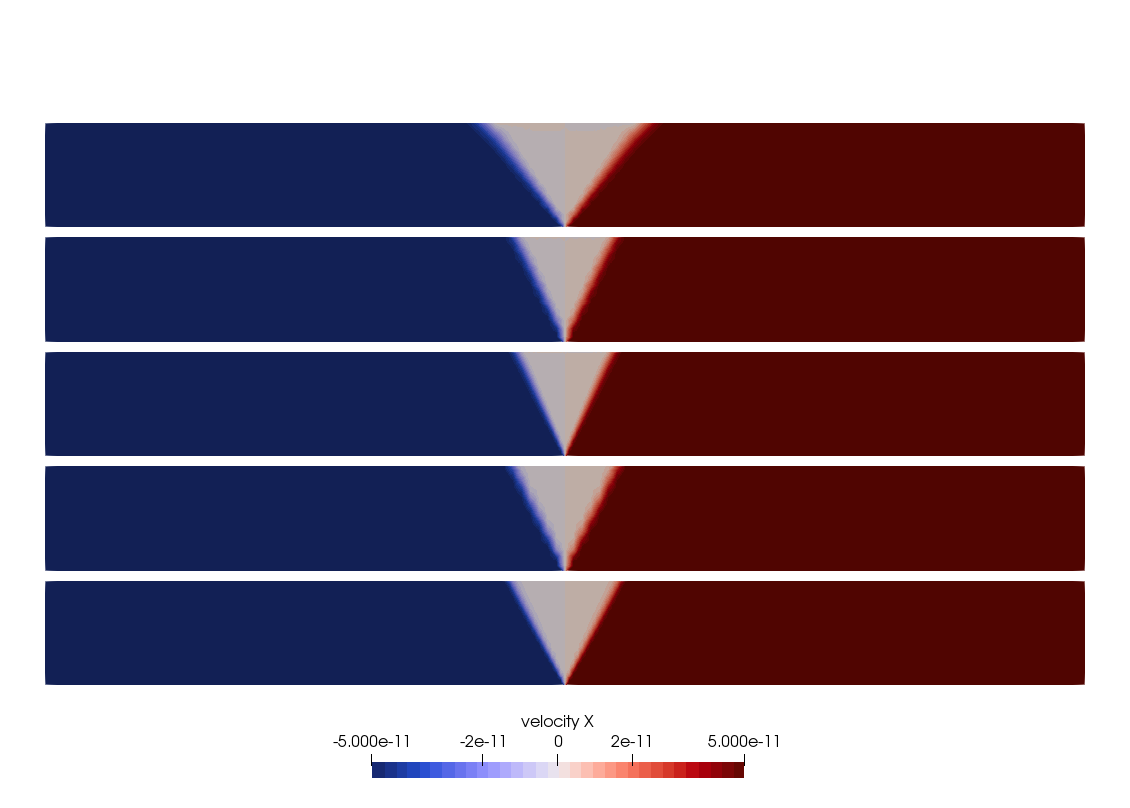
\includegraphics[width=.8\linewidth]{python_codes/fieldstone_39/images/extension_u}\\
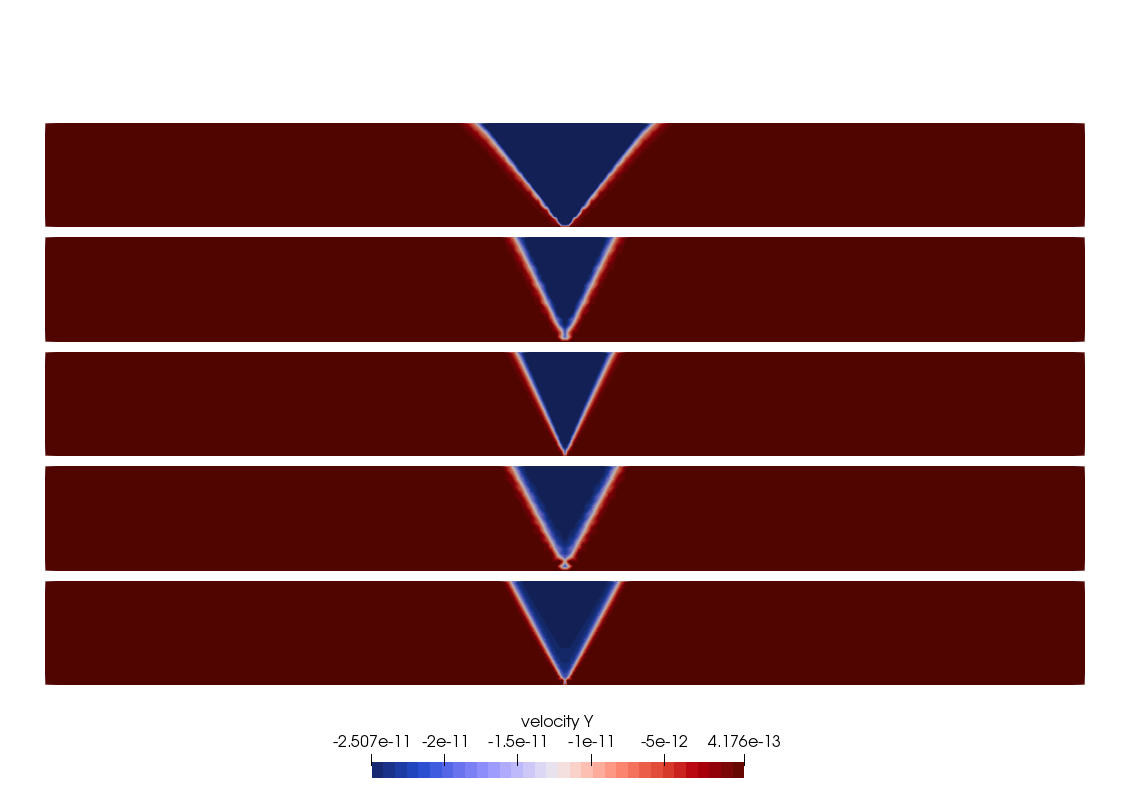
\includegraphics[width=.8\linewidth]{python_codes/fieldstone_39/images/extension_v}\\
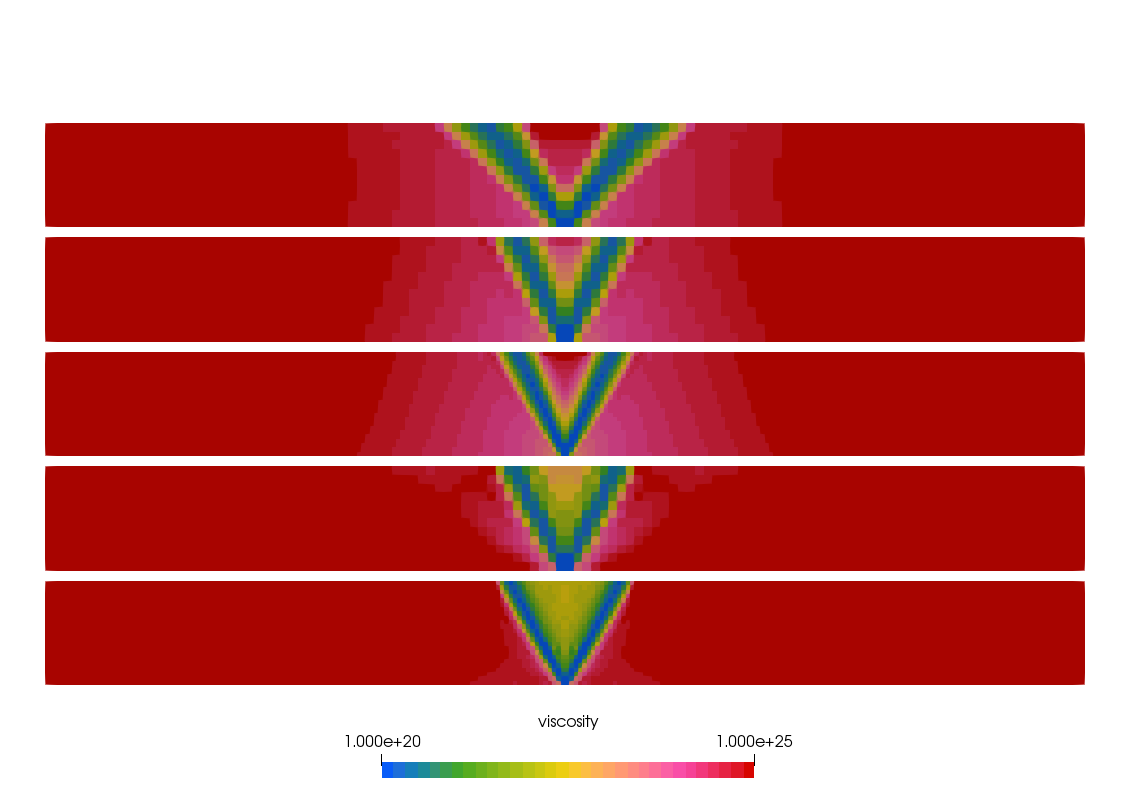
\includegraphics[width=.8\linewidth]{python_codes/fieldstone_39/images/extension_mueff}\\
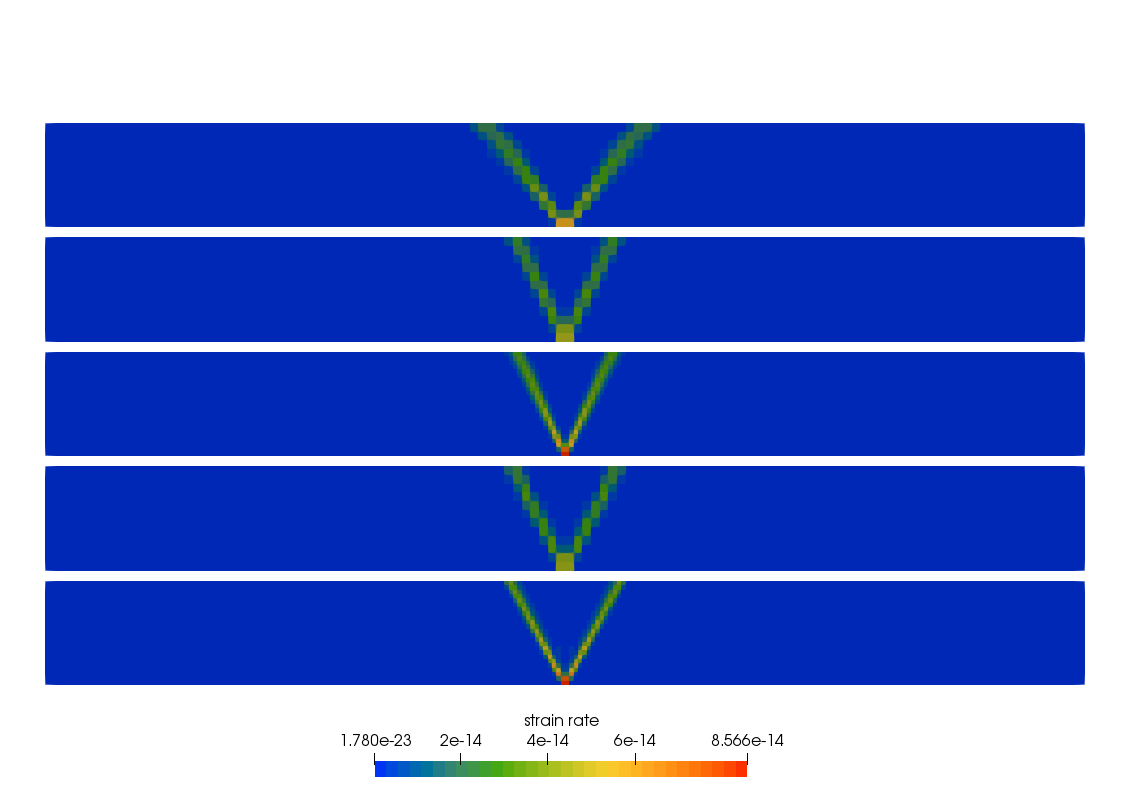
\includegraphics[width=.8\linewidth]{python_codes/fieldstone_39/images/extension_sr}\\
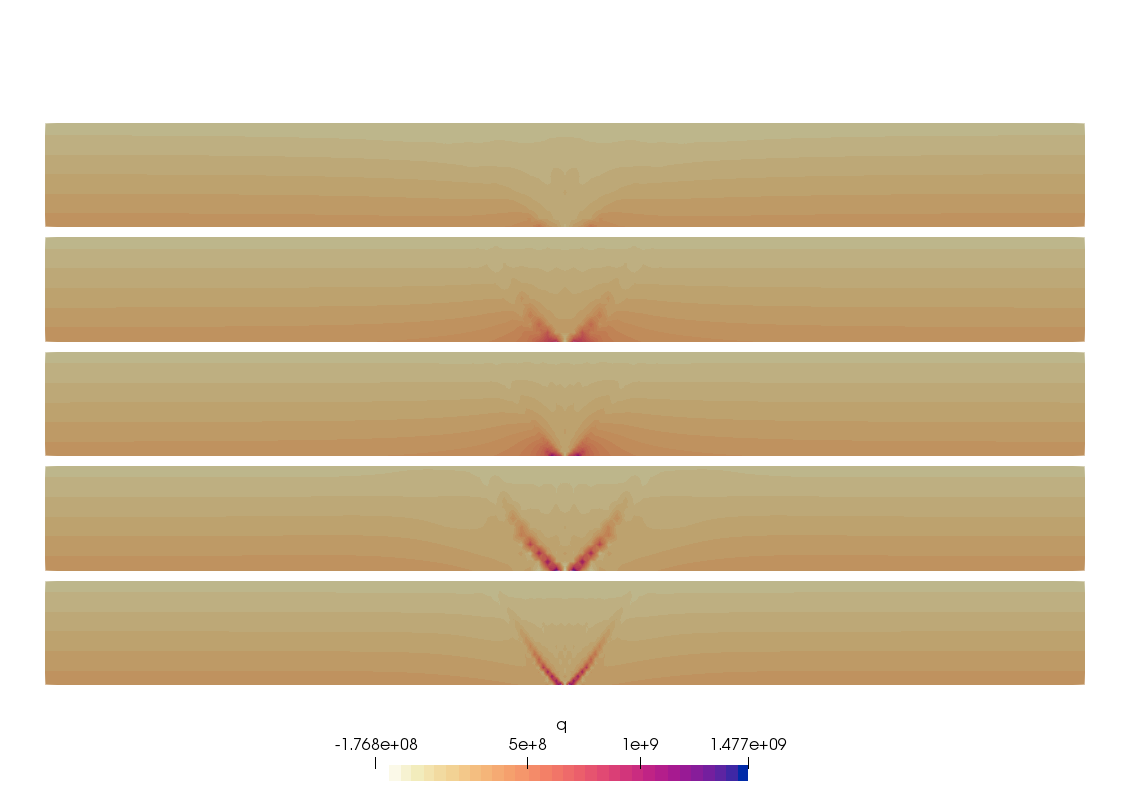
\includegraphics[width=.8\linewidth]{python_codes/fieldstone_39/images/extension_press}\\
{\small Extension. 1st row: Non-associative plasticity; 2nd and 3rd row: associative plasticity ($\psi=\phi$) with method 1 for two resolutions 120x12 and 240; 4th and 5th row: associative plasticity ($\psi=\phi$) with method 2 for two re    solutions 120x12 and 240}
\end{center}

\begin{center}
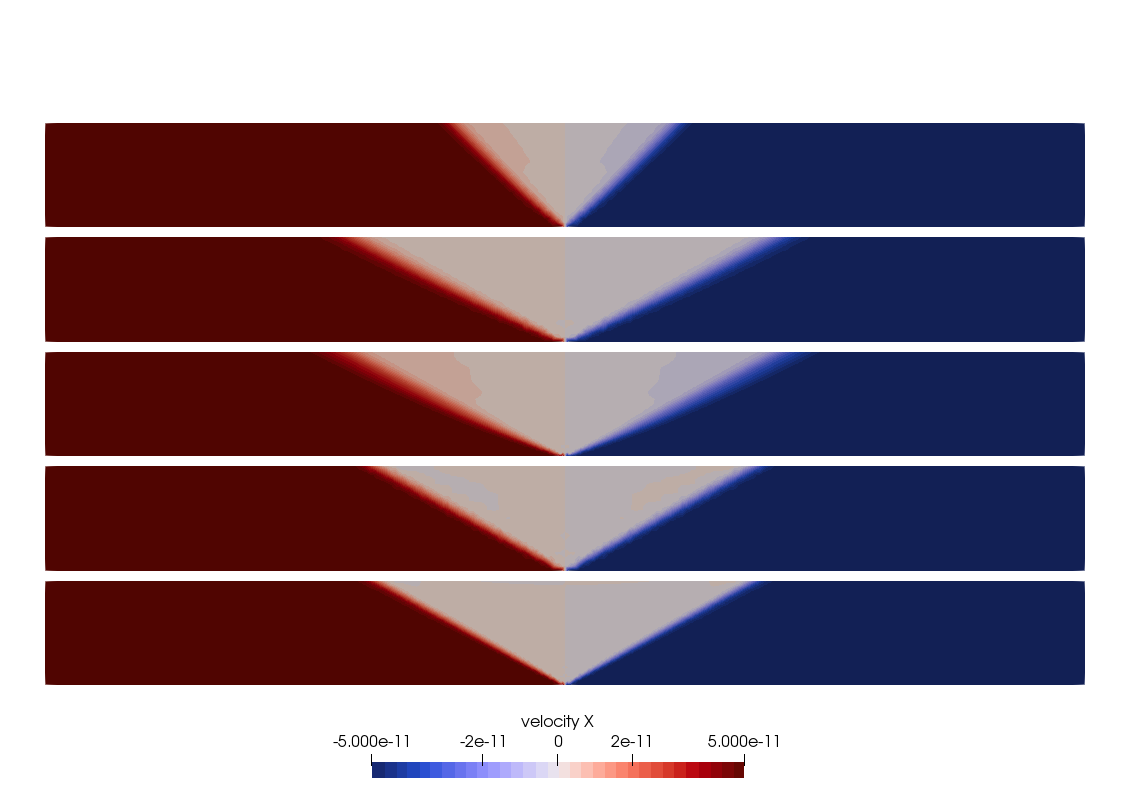
\includegraphics[width=.8\linewidth]{python_codes/fieldstone_39/images/compression_u}\\
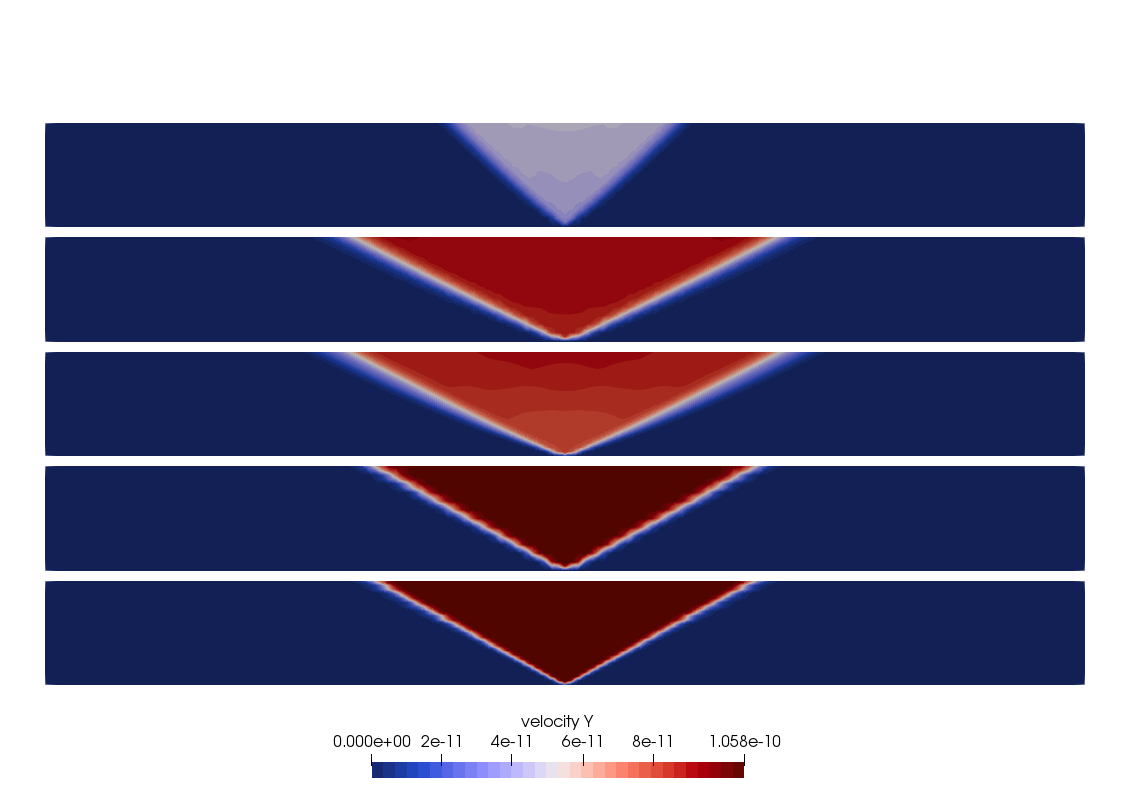
\includegraphics[width=.8\linewidth]{python_codes/fieldstone_39/images/compression_v}\\
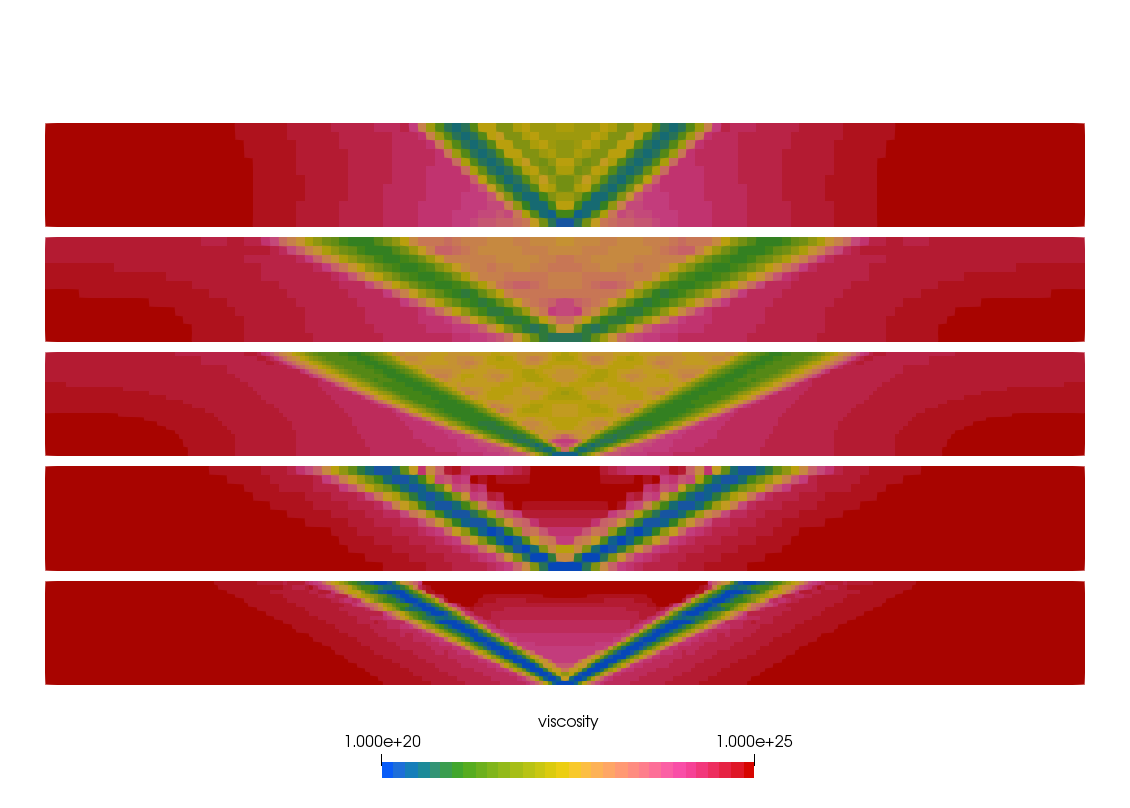
\includegraphics[width=.8\linewidth]{python_codes/fieldstone_39/images/compression_mueff}\\
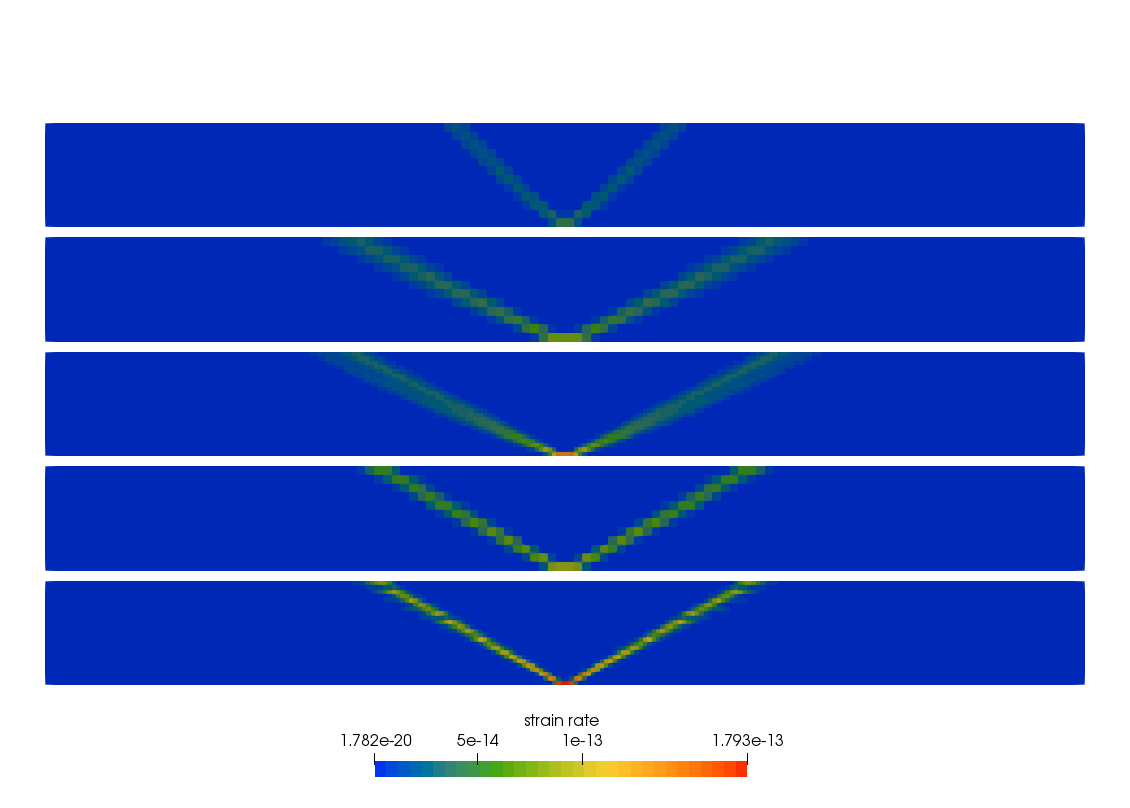
\includegraphics[width=.8\linewidth]{python_codes/fieldstone_39/images/compression_sr}\\
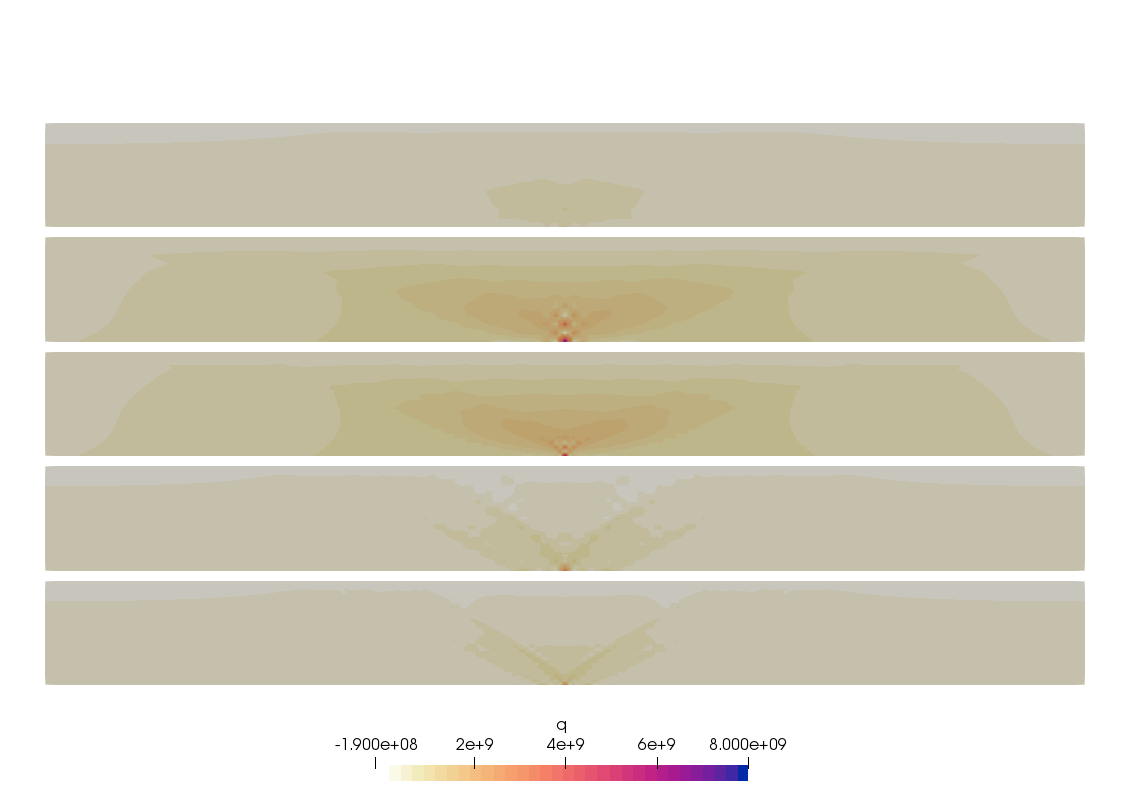
\includegraphics[width=.8\linewidth]{python_codes/fieldstone_39/images/compression_press}\\
{\small Compression. 1st row: Non-associative plasticity; 2nd and 3rd row: associative plasticity ($\psi=\phi$) with method 1 for two resolutions 120x12 and 240; 4th and 5th row: associative plasticity ($\psi=\phi$) with method 2 for two re    solutions 120x12 and 240}
\end{center}


\begin{center}
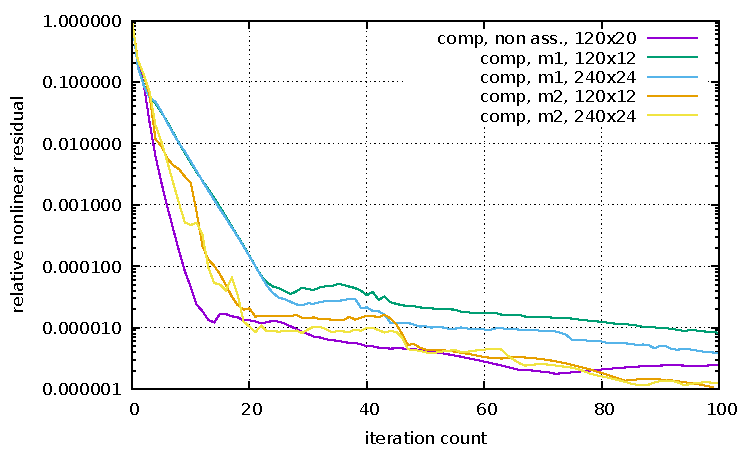
\includegraphics[width=.5\linewidth]{python_codes/fieldstone_39/images/conv_compression}
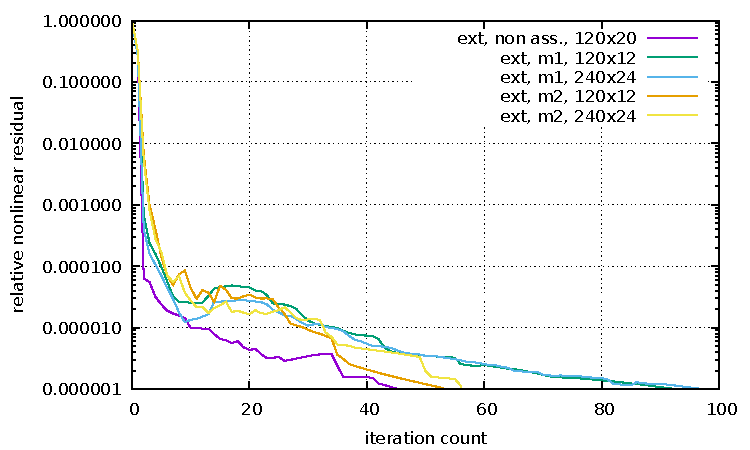
\includegraphics[width=.5\linewidth]{python_codes/fieldstone_39/images/conv_extension}
\end{center}

One can also run the extension model for $\phi=\psi={0,5,10,15,20,25,30}\degree$
\begin{center}
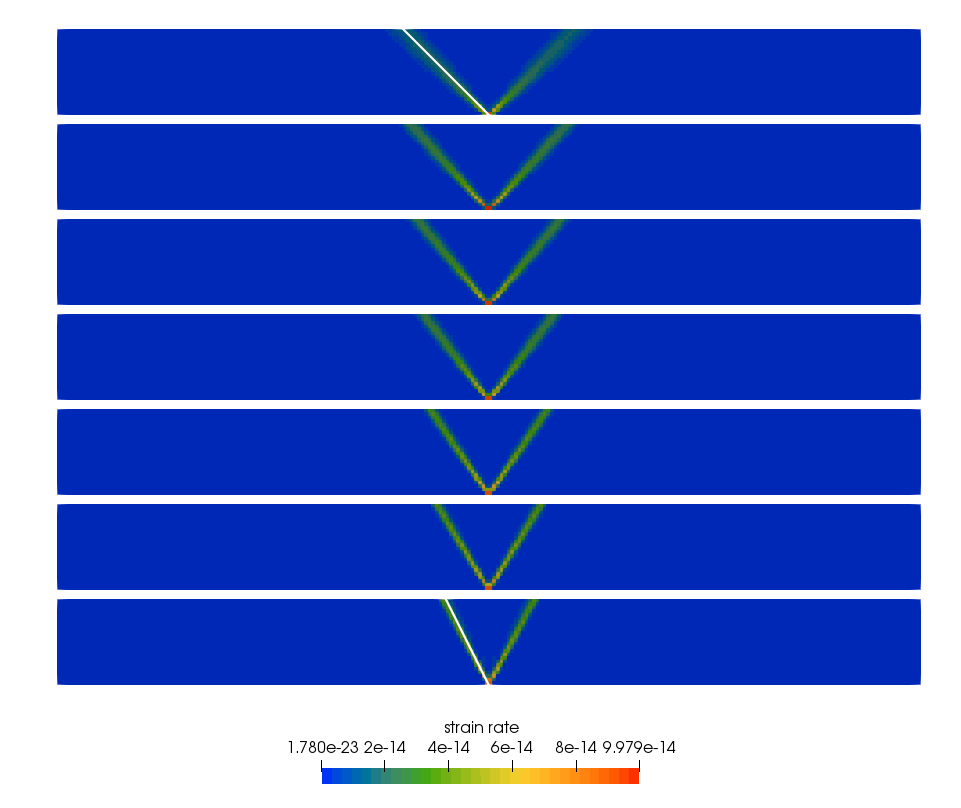
\includegraphics[width=.5\linewidth]{python_codes/fieldstone_39/images/sr_0_30}
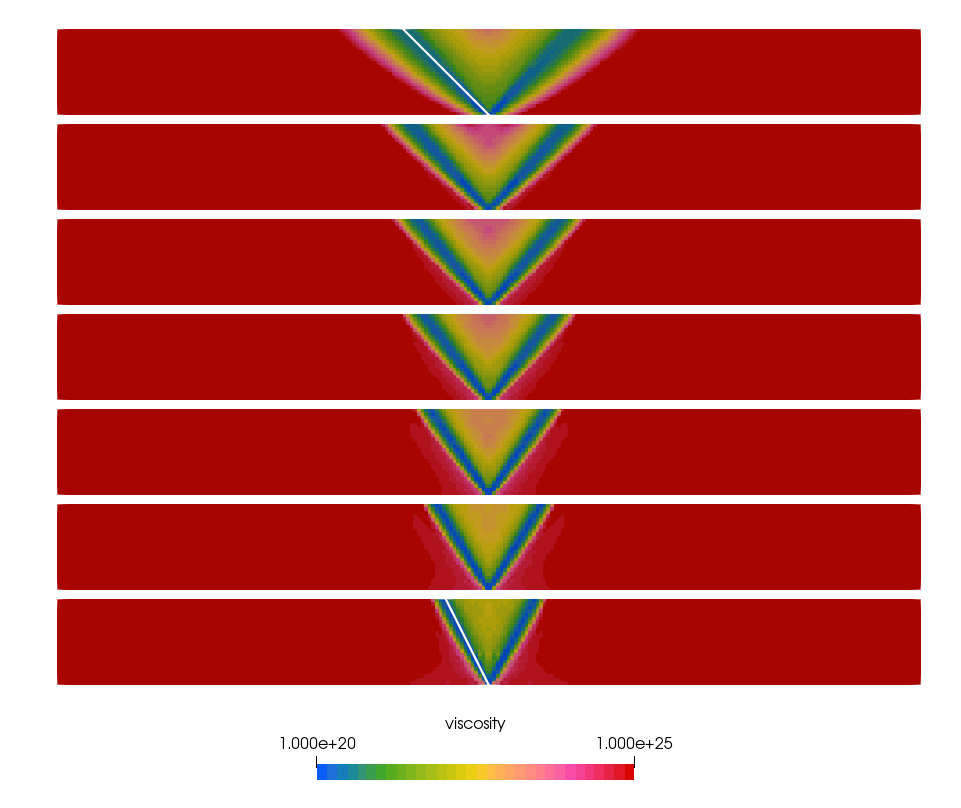
\includegraphics[width=.5\linewidth]{python_codes/fieldstone_39/images/etaeff_0_30}\\
\end{center}

Three angles are mechanically stable (e.g. \cite{kaus10}):
\[
\theta=\frac{\pi}{4}\pm \frac{\psi}{2} \qquad \text{Roscoe angle}
\]
\[
\theta=\frac{\pi}{4}\pm \frac{\phi}{2} \qquad \text{Coulomb angle}
\]
\[
\theta=\frac{\pi}{4}\pm \frac{\phi+\phi}{4} \qquad \text{Arthur angle}
\]
In the case of associative plasticity, $\phi=\psi$, so that all three angles are the same. 
Per row of elements, and per half of the domain (left and right) we find the element
with the highest strain-rate and record their center coordinates on the figure hereunder. 
These elements are shown for $\phi=\psi=\{0,10,20,30\}\degree$ alongside a line corresponding to 
the expected analytical shear band angle value.
\begin{center}
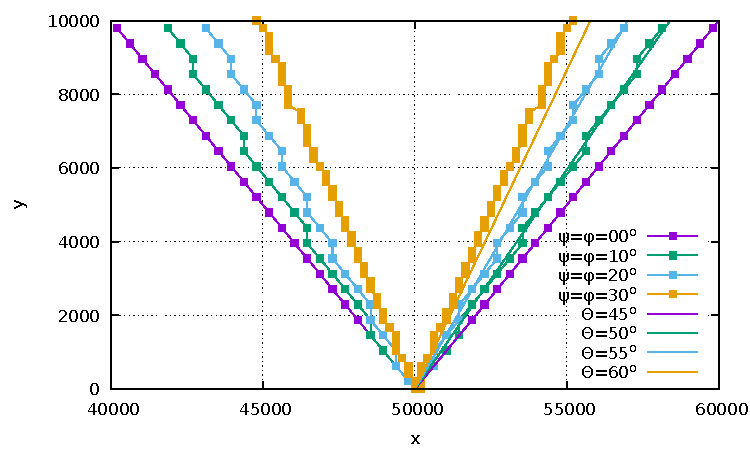
\includegraphics[width=.6\linewidth]{python_codes/fieldstone_39/images/shear_bands}\\
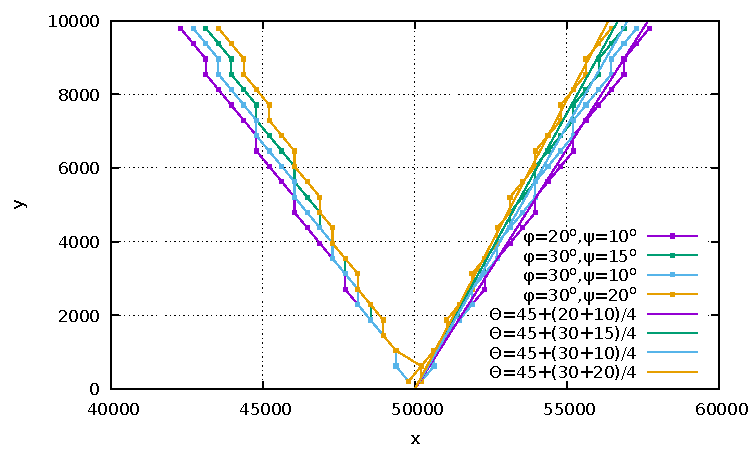
\includegraphics[width=.6\linewidth]{python_codes/fieldstone_39/images/shear_bands_nonass}\\
Results obtained on a 240x24 grid, max 50 nl iterations.
\end{center}



Note that benchmarking this in not easy. One solution Timo and I found was to add a 
velocity field $\underline{\vec\upnu}=(x,y,z)$ (with $\vec\nabla\cdot\underline{\vec\upnu}=3$)
to an existing analytical problem, e.g. the Burstedde benchamrk.

%..........................................................
\subsubsection*{The 2016 brick}

The setup is similar to the one in \cite{spmw16}. It is a 2D Cartesian domain filled with an 
isoviscous layer at the bottom and a visco-plastic material on top, as shown here:  

%\begin{center}
%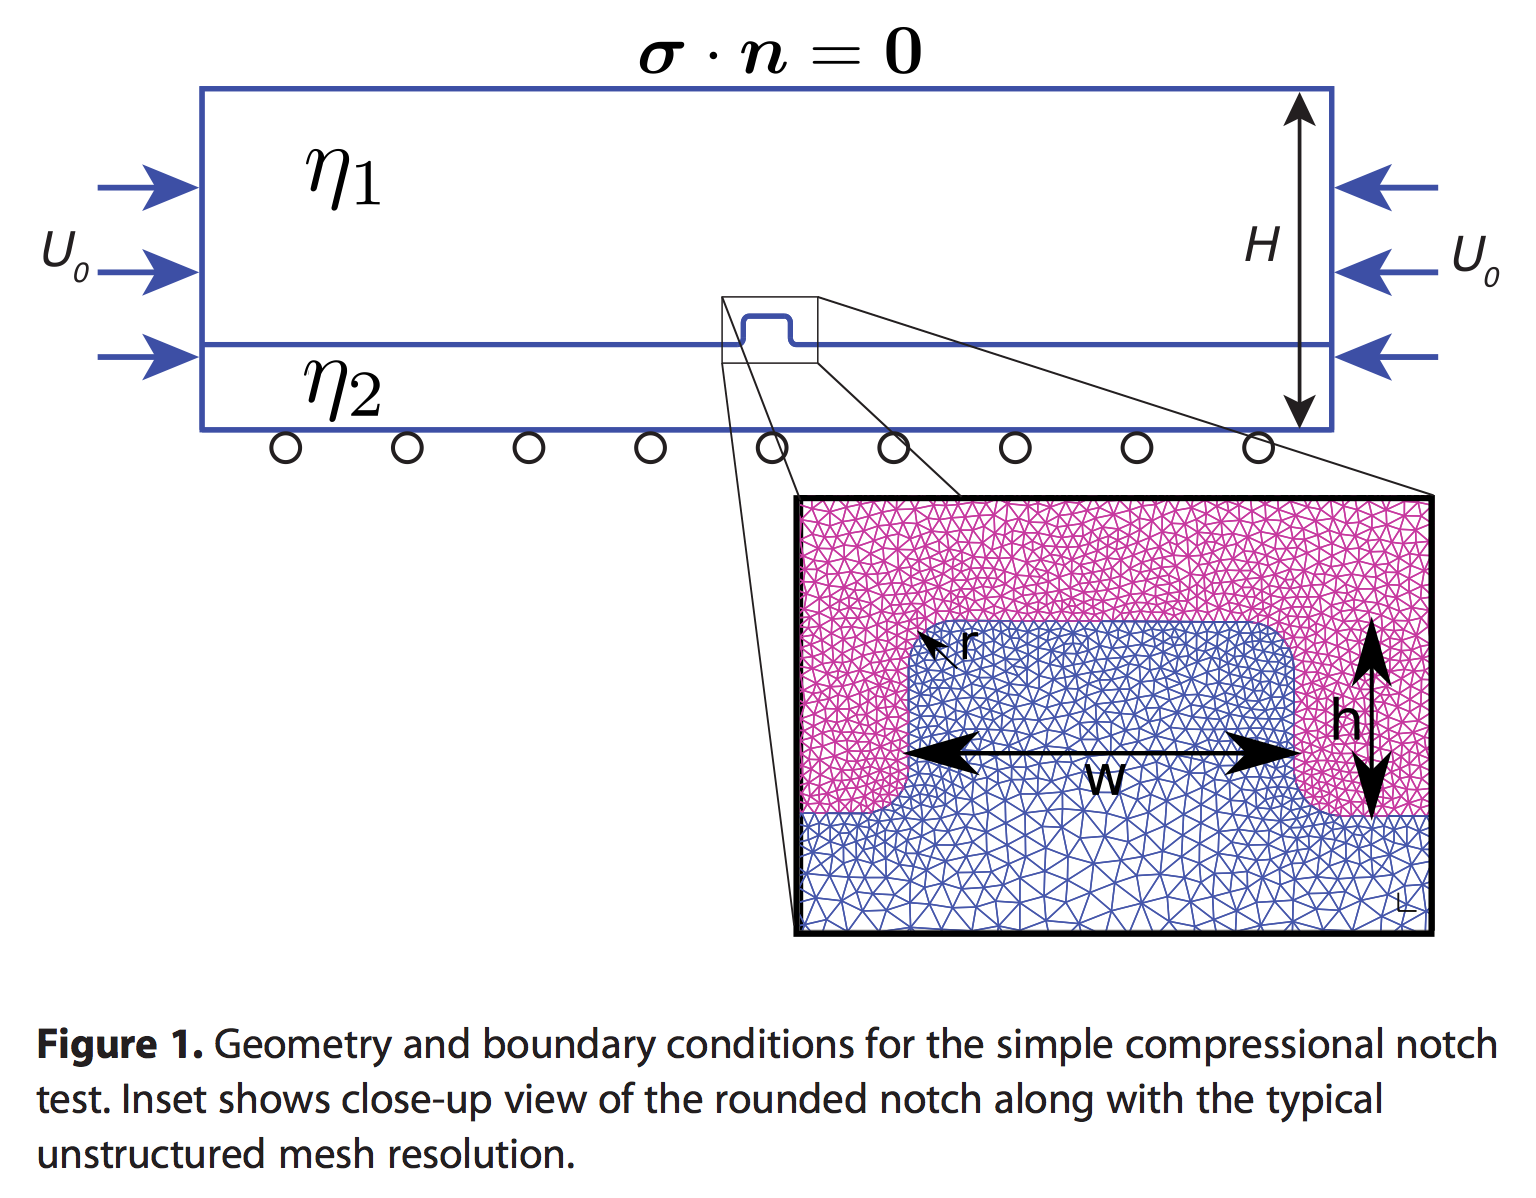
\includegraphics[width=6cm]{python_codes/fieldstone_39/images/spmw_1.png}
%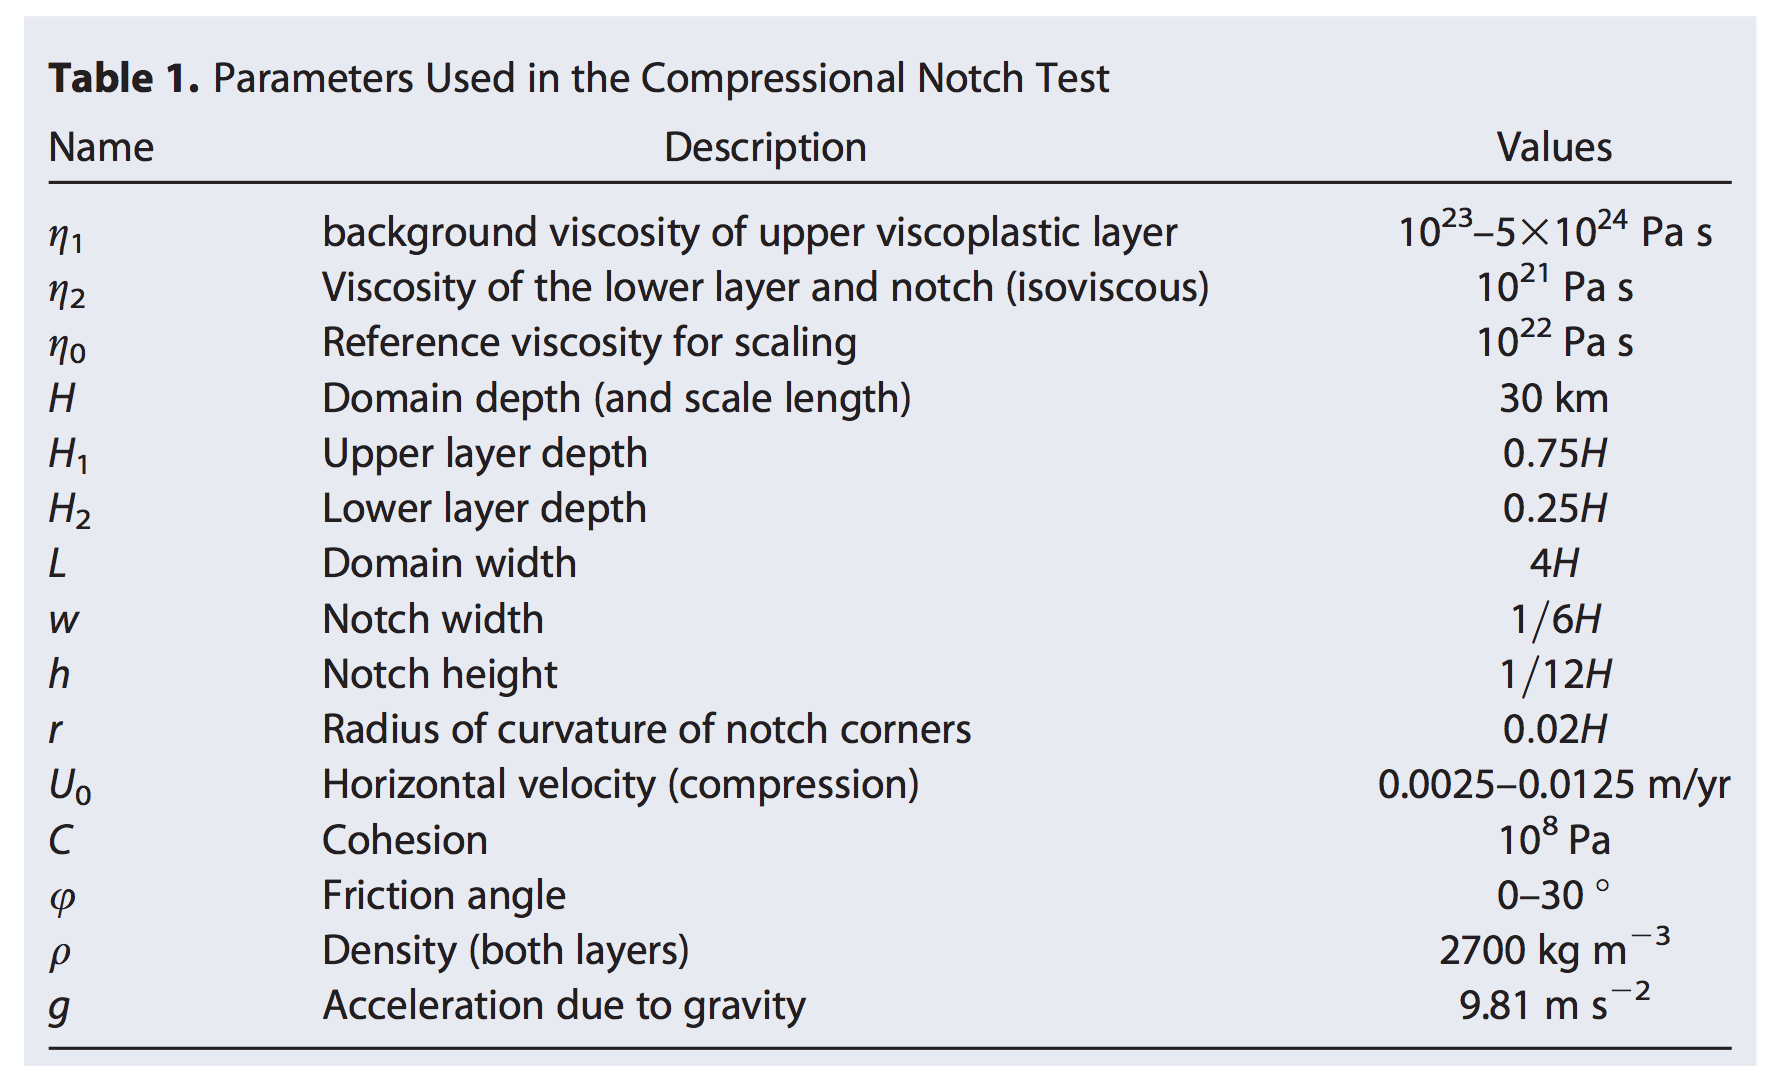
\includegraphics[width=8cm]{python_codes/fieldstone_39/images/spmw_2.png}
%\end{center}


In what follows the nonlinear tolerance is set to $10^{-6}$. Due to a lack of resolution, I do not
implement the rounded edges of the seed. $U_0$ is set to 25mm/yr and the background viscosity of the brittle layer
is set to $\eta_0=10^{24}$Pa.s. Note that the effective viscosity of the brittle layer is computed as follows:
\[
\eta_{eff}
=\left( \frac{1}{\eta_0} + \frac{1}{\eta_p}  \right)^{-1}
=\left( \frac{1}{\eta_0} + \frac{2 \dot{\epsilon}_{ii}}{Y}  \right)^{-1}
\]
with $Y=p \sin \phi + c \cos \phi$. 
Note that the pressure colour bars in Fig(6) of \cite{spmw16} are most likely not correct at all, 
and in order for my results to look like theirs I had to change it for VM, DDM and DP. 

%\begin{center}
%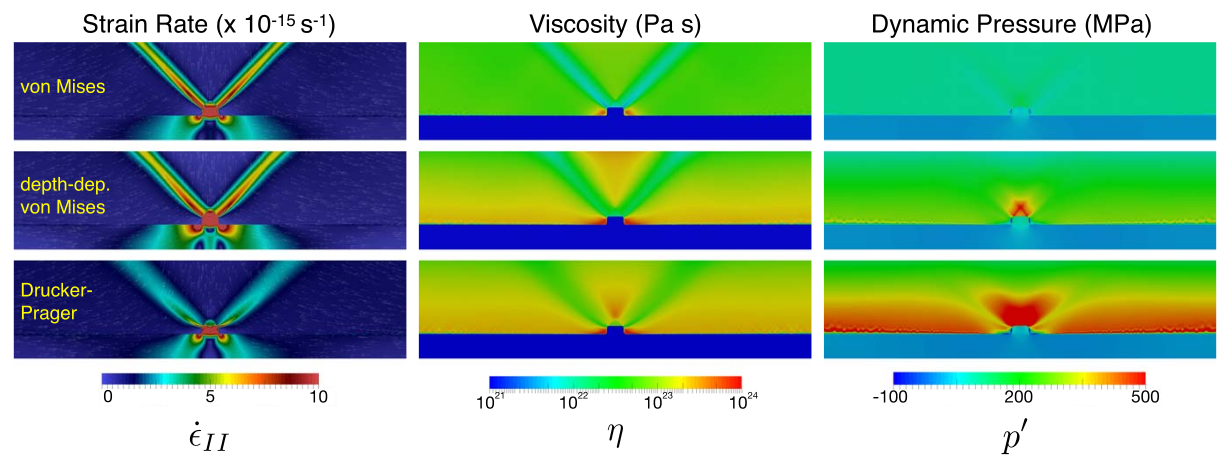
\includegraphics[width=12cm]{python_codes/fieldstone_39/images/spmw_3.png}\\
%{\small Results from Spiegelman et al \cite{spmw16}}
%\end{center}

%\begin{center}
%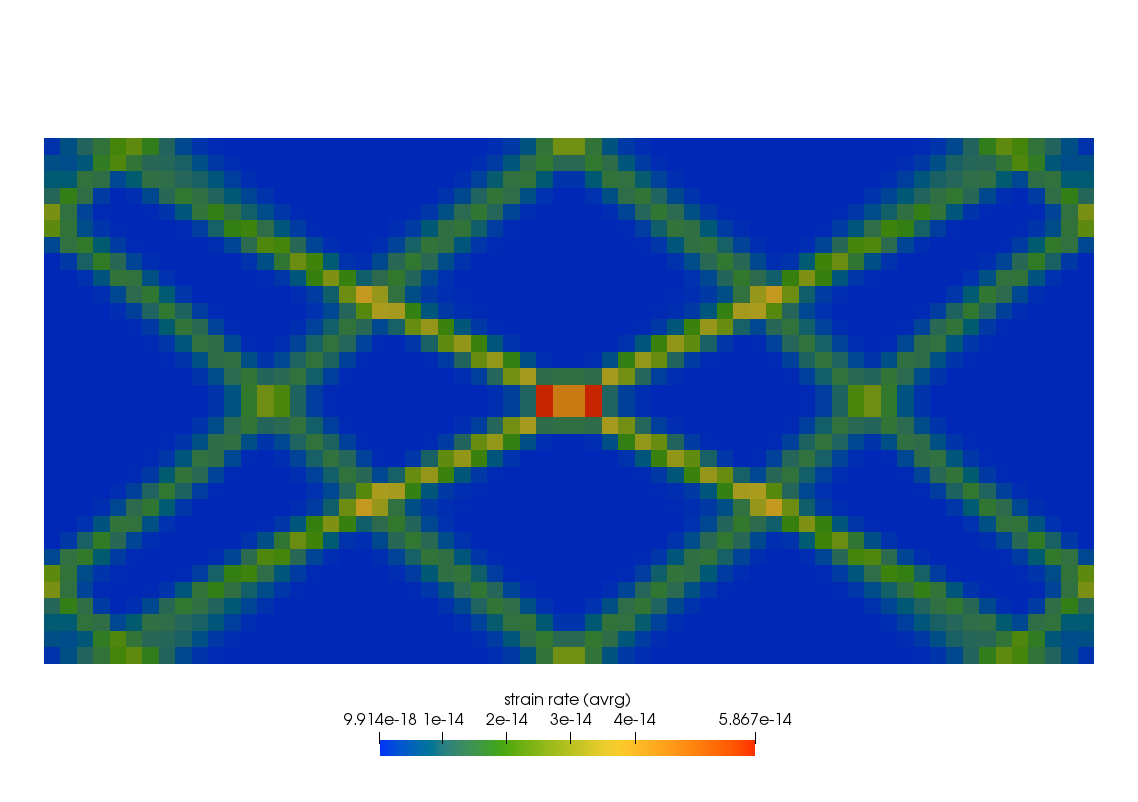
\includegraphics[width=5cm]{python_codes/fieldstone_39/poster/new_spmw16_lvl3_vM/sr}
%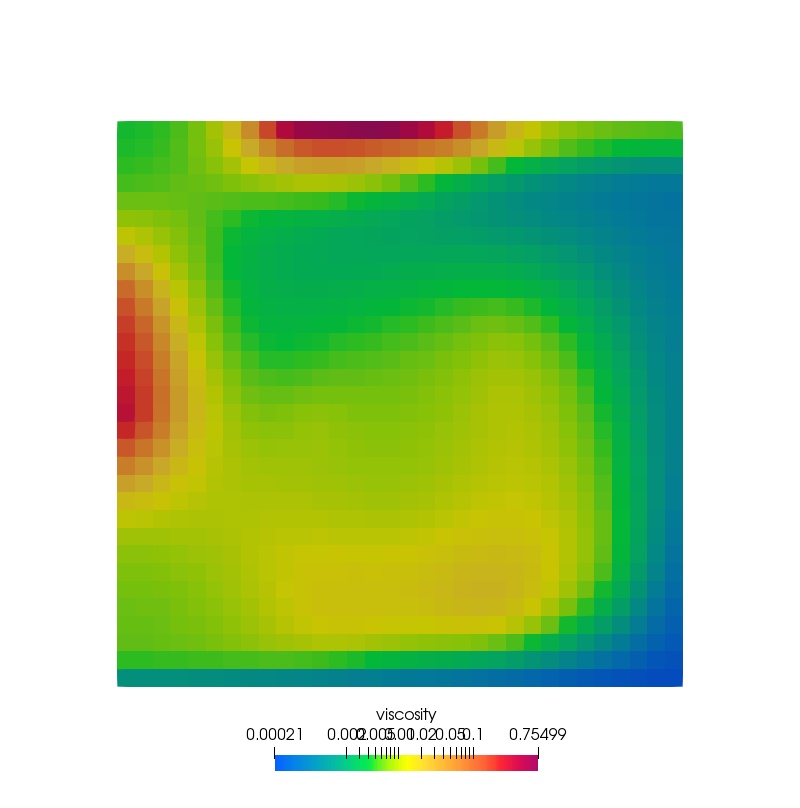
\includegraphics[width=5cm]{python_codes/fieldstone_39/poster/new_spmw16_lvl3_vM/mueff}
%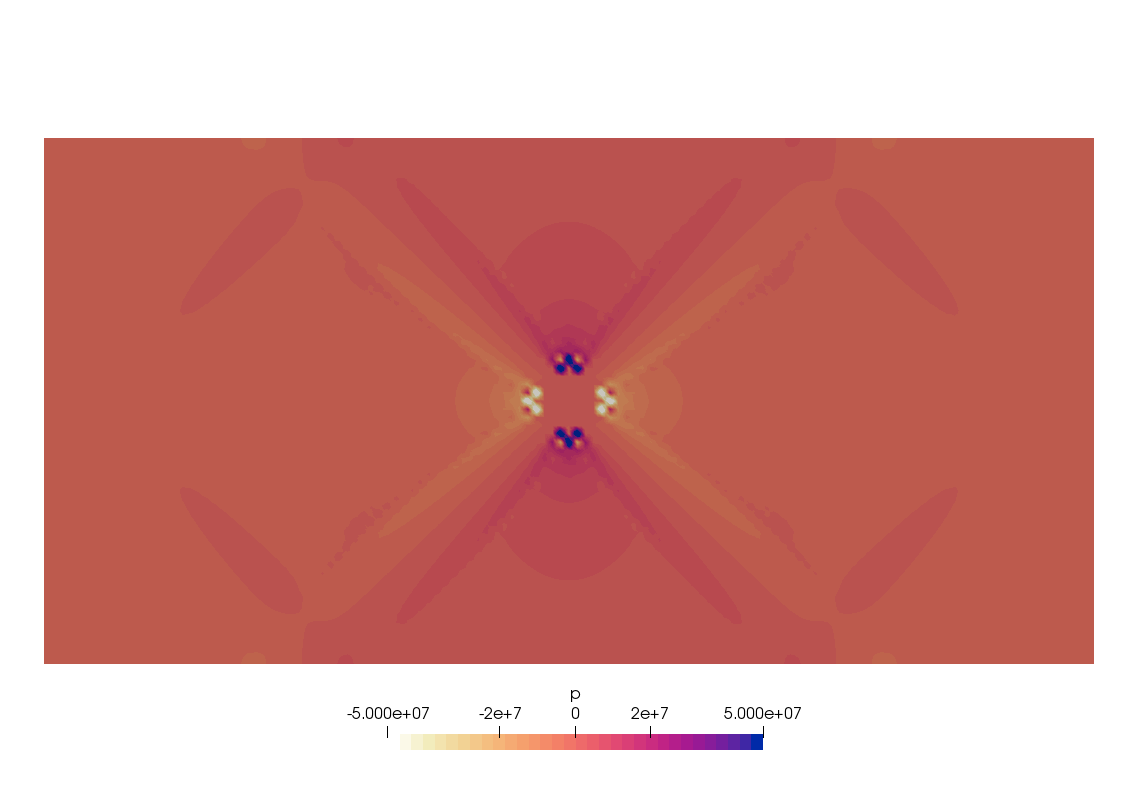
\includegraphics[width=5cm]{python_codes/fieldstone_39/poster/new_spmw16_lvl3_vM/p}\\
%{\small von Mises case, results with fieldstone, lvl 3}
%\end{center}


%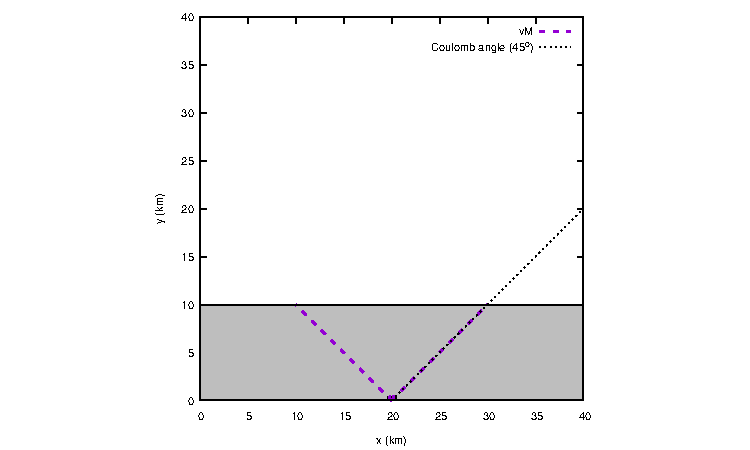
\includegraphics[width=5cm]{python_codes/fieldstone_39/poster/shear_bands_vM.pdf}
%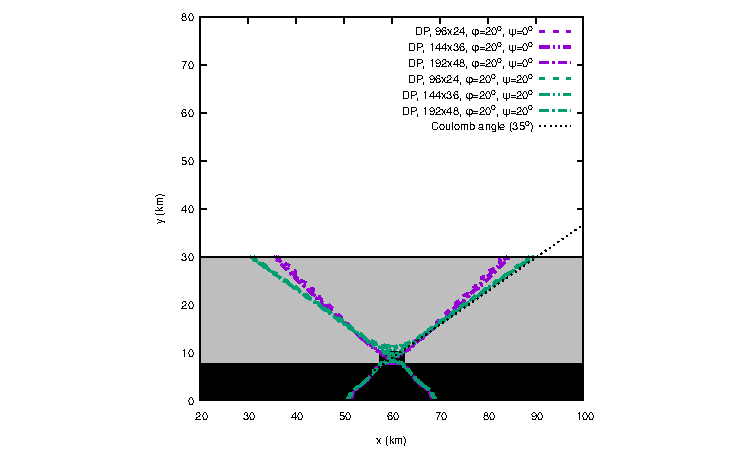
\includegraphics[width=5cm]{python_codes/fieldstone_39/poster/shear_bands_DP20.pdf}
%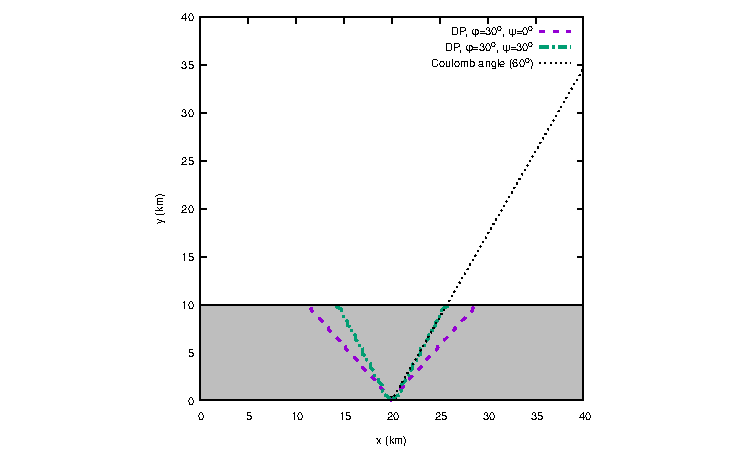
\includegraphics[width=5cm]{python_codes/fieldstone_39/poster/shear_bands_DP30.pdf}

%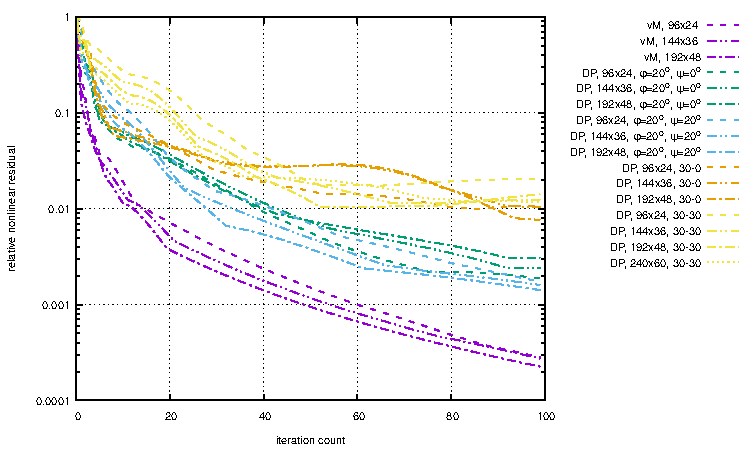
\includegraphics[width=7cm]{python_codes/fieldstone_39/poster/nonlinear_conv.pdf}

